\let\negmedspace\undefined
\let\negthickspace\undefined
\documentclass[journal]{IEEEtran}
\usepackage[a5paper, margin=10mm, onecolumn]{geometry}
\usepackage{lmodern} 
\usepackage{tfrupee} 
\setlength{\headheight}{1cm}
\setlength{\headsep}{0mm}   

\usepackage{gvv-book}
\usepackage{gvv}
\usepackage{cite}
\usepackage{amsmath,amssymb,amsfonts,amsthm}
\usepackage{algorithmic}
\usepackage{graphicx}
\usepackage{textcomp}
\usepackage{xcolor}
\usepackage{txfonts}
\usepackage{listings}
\usepackage{enumitem}
\usepackage{mathtools}
\usepackage{gensymb}
\usepackage{comment}
\usepackage[breaklinks=true]{hyperref}
\usepackage{tkz-euclide} 
\usepackage{listings}                             
\def\inputGnumericTable{}                                 
\usepackage[latin1]{inputenc}                                
\usepackage{color}                                            
\usepackage{array}                                            
\usepackage{longtable}                                       
\usepackage{calc}                                             
\usepackage{multirow}                                         
\usepackage{hhline}                                           
\usepackage{ifthen}                                           
\usepackage{lscape}
\usepackage{xparse}

\bibliographystyle{IEEEtran}

\title{1.10.30}
\author{EE25BTECH11062 - Vivek K Kumar}

\begin{document}
\maketitle

\renewcommand{\thefigure}{\theenumi}
\renewcommand{\thetable}{\theenumi}

\numberwithin{equation}{enumi}
\numberwithin{figure}{enumi} 

\textbf{Question}:\\
The direction cosines of the vector \myvec{2 \\ 2 \\ -1} are \underline{\hspace{0.1\columnwidth}}
\\
\textbf{Solution: }
\begin{table}[H]    
  \centering
  \begin{tabular}{|c|c|}
\hline
\textbf{Name} & \textbf{Value} \\ \hline
$\vec{A}$ & $\myvec{2 & 1 \\0 & 3}$ \\ \hline
\end{tabular}

  \caption{Variables Used}
  \label{tab:1.10.30}
\end{table}
The unit vector along the direction of given vector is\\
\begin{align}
  \frac{\vec{A}}{\norm{\vec{A}}} &= \frac{1}{3}\myvec{2 \\ 2 \\ -1} \\
 &=\myvec{\frac{2}{3} \\ \frac{2}{3} \\ \frac{-1}{3}}
\end{align}
\begin{figure}[H]
   \centering
  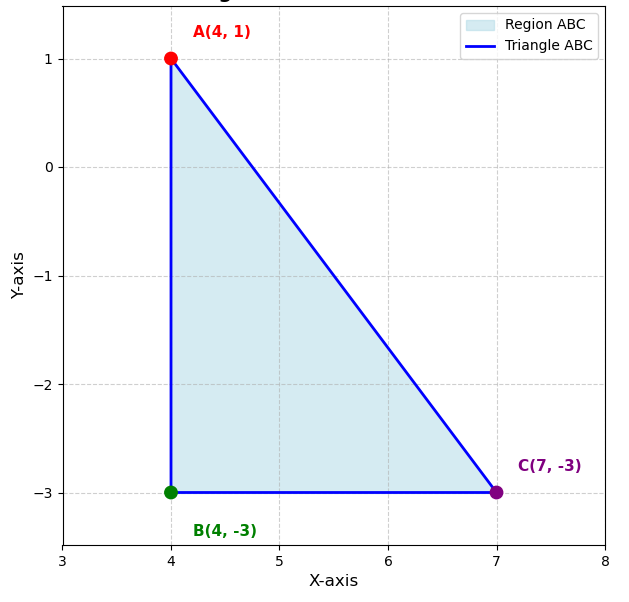
\includegraphics[width=0.64\columnwidth]{figs/fig.png}
   \caption{Given vector and its direction cosines}
   \label{stemplot}
\end{figure}
\end{document}  

